\vspace{-1em}
\section{Programming Model}
\vspace{-0.4em}

\label{sec:programming_model}
This section introduces the \lang programming model with a running example, describes its language primitives and execution modes, and outlines runtime optimization opportunities.
This programming model can simplify tedious operations in multi-call workflows (e.g., string manipulation, API calling, constraint specification, parallelism) by providing flexible and composable primitives.

\begin{figure}[t]
\centering
\vspace{-2.5em}
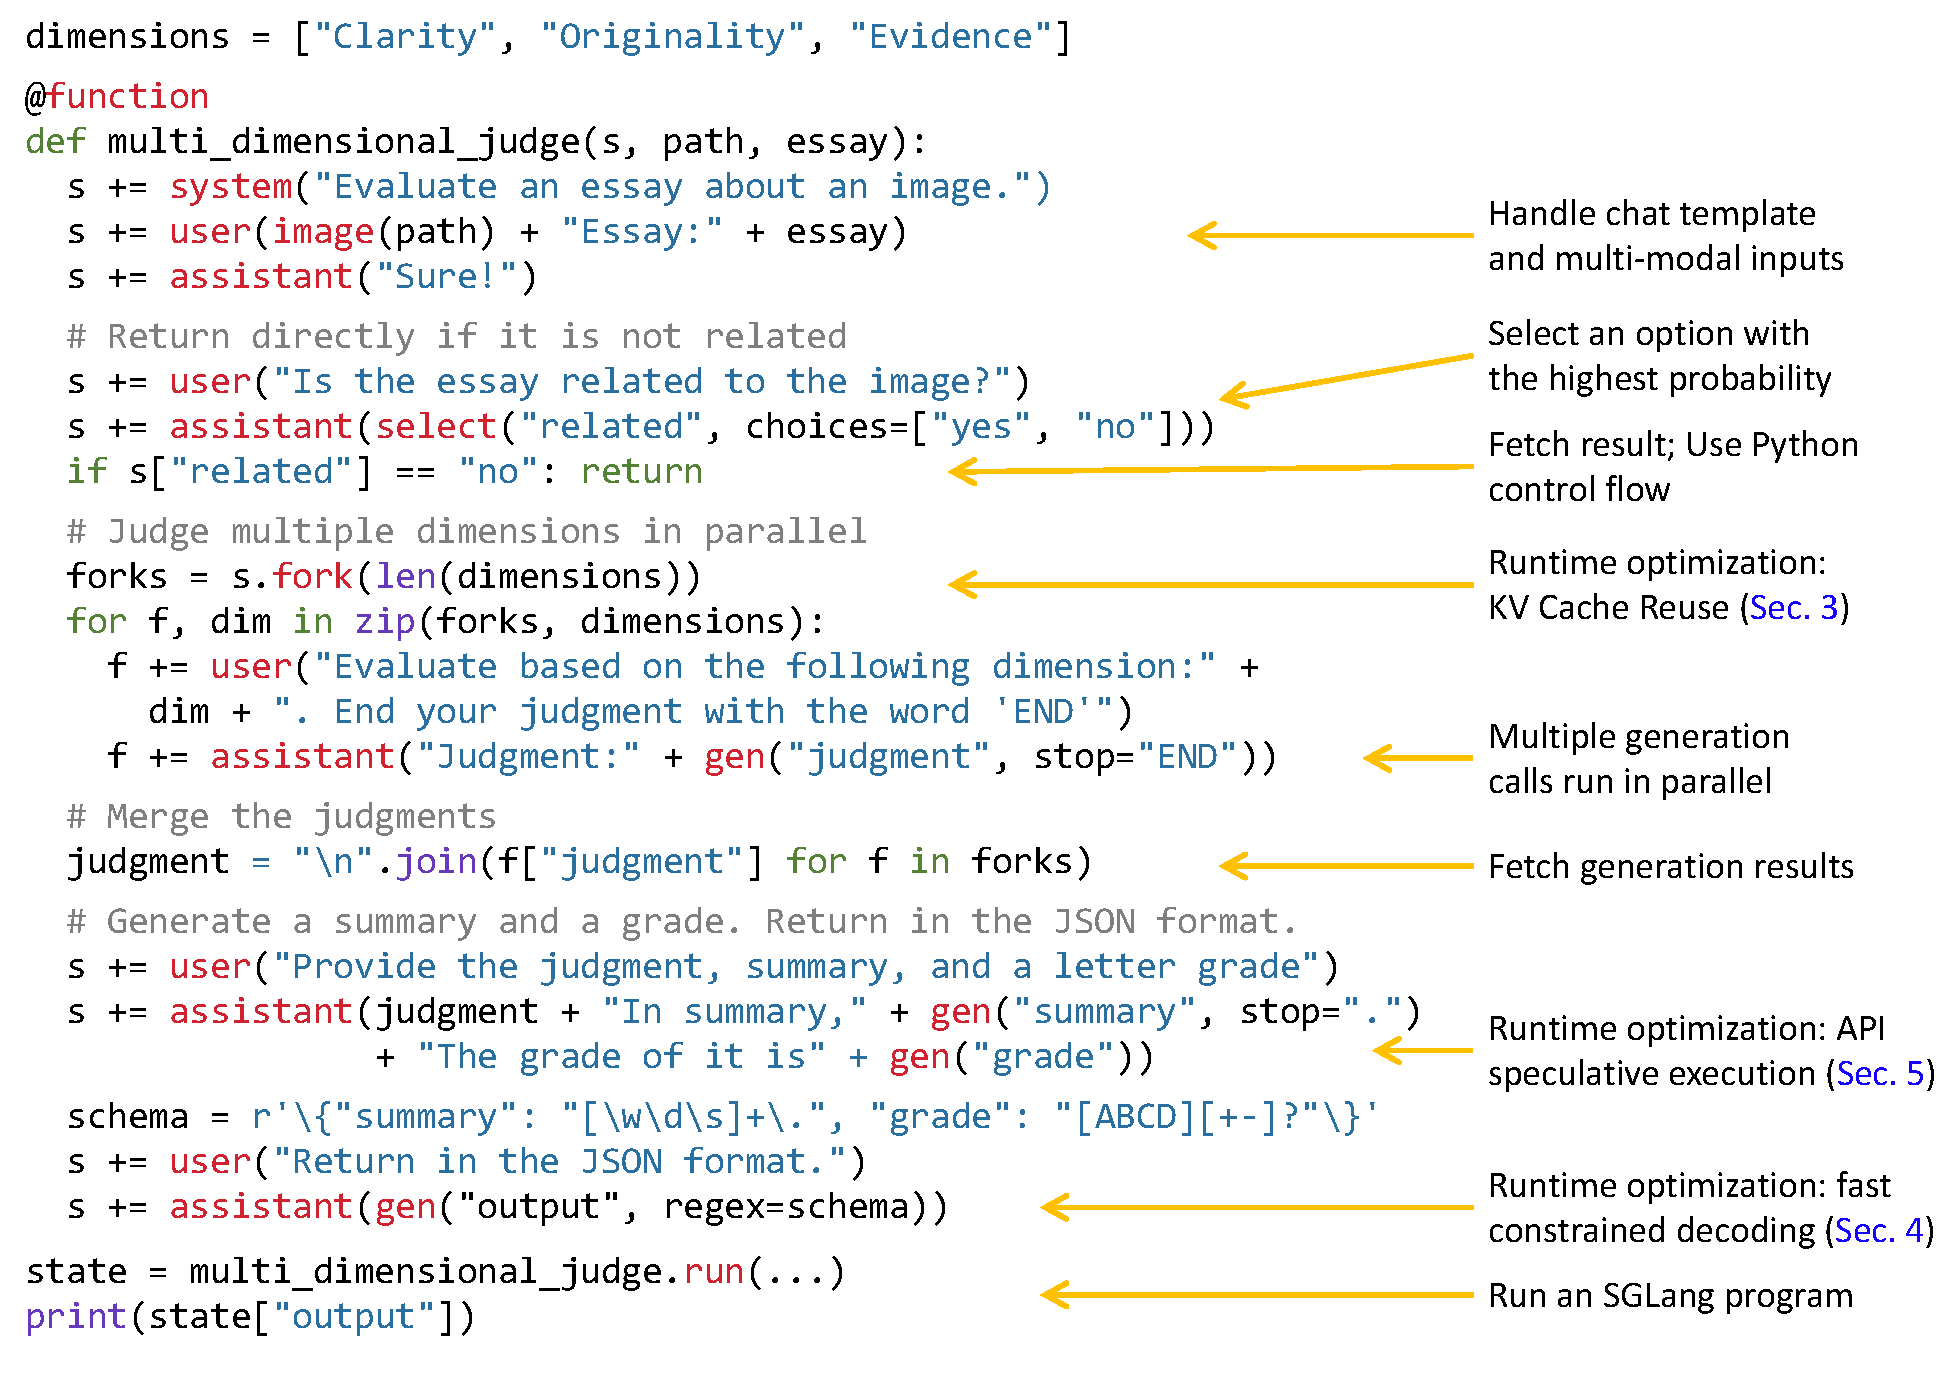
\includegraphics[width=0.97\linewidth]{figures/example_first_program.pdf}
\vspace{-1em}
\caption{\small
The implementation of a multi-dimensional essay judge in \lang utilizes the branch-solve-merge prompting technique~\cite{saha2023branch}. Primitives provided by \lang are shown in red.}
\vspace{-1em}
\label{fig:example_first_program}
\end{figure}

\textbf{A running example.} 
The language is a domain-specific language embedded in Python. 
\autoref{fig:example_first_program} shows a program that evaluates an essay about an image using the branch-solve-merge prompting method~\cite{saha2023branch}.
The function \texttt{multi\_dimensional\_judge} takes three arguments: \texttt{s}, \texttt{path}, and \texttt{essay}.
\texttt{s} manages the prompt state, \texttt{path} is the image file path, and \texttt{essay} is the essay text.
New strings and \lang primitives can be appended to the state \texttt{s} for execution using the \texttt{+=} operator.
First, the function adds the image and essay to the prompt.
It then checks if the essay is related to the image using \texttt{select}, storing the result in \texttt{s["related"]}.
If related, the prompt is forked into three copies for parallel evaluation from different dimensions, using \texttt{gen} to store results in \texttt{f["judgment"]}.
Next, it merges the judgments, generates a summary, and assigns a letter grade.
Finally, it returns the results in JSON format, following a schema defined by a regular expression constraint \texttt{regex}.
\lang greatly simplifies this program, as an equivalent program using an OpenAI API-like interface would take $2.1\times$ as many lines of code due to manual string manipulation and parallelism control.

\textbf{Language primitives.}
\lang provides primitives for controlling prompt state, generation, and parallelism. They can be used together with Python syntax and libraries.
Here are the primitives:
``\texttt{gen}'' calls a model to generate and stores the results in a variable with the name specified in its first argument. It supports a ``\texttt{regex}'' argument to constrain the output to follow a grammar defined by a regular expression (e.g., a JSON schema).
``\texttt{select}'' calls a model to choose the highest probability option from a list.
The operator ``\texttt{+=}'' or ``\texttt{extend}'' appends a string to the prompt.
The operator ``\texttt{[variable\_name]}'' fetches the results of a generation.
``\texttt{fork}'' creates parallel forks of the prompt state.
``\texttt{join}'' rejoins the prompt state.
``\texttt{image}'' and ``\texttt{video}'' take in image and video inputs.

\textbf{Execution modes.}
The simplest way to execute an \lang program is through an interpreter, where a prompt is treated as an asynchronous stream. Primitives like \texttt{extend}, \texttt{gen}, and \texttt{select} are submitted to the stream for asynchronous execution. These non-blocking calls allow Python code to continue running without waiting for the generation to finish. This is similar to launching CUDA kernels asynchronously. Each prompt is managed by a stream executor in a background thread, enabling intra-program parallelism. Fetching generation results will block until they are ready, ensuring correct synchronization.
Alternatively, \lang programs can be compiled as computational graphs and executed with a graph executor, allowing for more optimizations. This paper uses interpreter mode by default and discusses compiler mode results in \autoref{sec:compiler_mode}.
\lang supports open-weight models with its own \lang Runtime (SRT), as well as API models such as OpenAI and Anthropic models.

\textbf{Comparison.}
Programming systems for LLMs can be classified as high-level (e.g., LangChain, DSPy) and low-level (e.g., LMQL, Guidance, \lang).
High-level systems provide predefined or auto-generated prompts, such as DSPy's prompt optimizer.
Low-level systems typically do not alter prompts but allow direct manipulation of prompts and primitives.
\lang is a low-level system similar to LMQL and Guidance. \autoref{tab:diff_lang} compares their features.
\lang focuses more on runtime efficiency and comes with its own co-designed runtime, allowing for novel optimizations introduced later.
High-level languages (e.g., DSPy) can be compiled to low-level languages (e.g., \lang).
We demonstrate the integration of \lang as a backend in DSPy for better runtime efficiency in \autoref{sec:eval}.


\textbf{Runtime optimizations.}
\autoref{fig:example_first_program} shows three runtime optimization opportunities: KV cache reuse, fast constrained decoding, API speculative execution. We will discuss them in the following sections.

\begin{table*}[t]
\footnotesize
    \centering
     \vspace{-2.5em}
    \caption{\small Comparison among LMQL, Guidance, and \lang.}
     \vspace{-0.9em}
    \resizebox{0.9\columnwidth}{!}{
    \begin{tabular}{llll}
    \toprule
    System & Syntax & Language Primitives & Runtime Backends \\
    \midrule
    LMQL     & Custom & extend, gen, select        & HF Transformers, llama.cpp, OpenAI \\
    Guidance & Python & extend, gen, select, image & HF Transformers, llama.cpp, OpenAI \\
    \midrule
    \lang    & Python & extend, gen, select, image, video, fork, join &  \lang Runtime (SRT), OpenAI\\
    \bottomrule
    \end{tabular}
    }
    \vspace{-2em}
    \label{tab:diff_lang}
\end{table*}



